\chapter{Implémentation}
\label{chap:implementation}

\section{Environnement technique}

L'ensemble a été développé sous GNU/Linux (Ubuntu, via WSL sur Windows). La
chaîne d'outils est entièrement libre :

\begin{table}[ht]
\centering
\caption{Outils et versions employés.}
\begin{tabular}{@{}ll@{}}
\toprule
\textbf{Outil} & \textbf{Rôle} \\
\midrule
GCC & compilateur C (et assembleur \code{-m32} pour l'extension) \\
GNU Bison 3.8 & générateur d'analyseur syntaxique LALR(1) \\
Flex 2.6 & générateur d'analyseur lexical \\
GNU Make & automatisation de la compilation \\
Valgrind & détection des fuites et erreurs mémoire \\
\TeX{} Live & rédaction du présent rapport \\
\bottomrule
\end{tabular}
\end{table}

\section{Architecture logicielle}

\subsection{Organisation du code}

Le code est découpé en modules à responsabilité unique, listés dans le
tableau~\ref{tab:fichiers}. Cette séparation reflète directement le pipeline de la
figure~\ref{fig:pipeline}.

\begin{table}[ht]
\centering
\caption{Modules du projet et leur rôle.}
\label{tab:fichiers}
\begin{tabular}{@{}ll@{}}
\toprule
\textbf{Fichier} & \textbf{Responsabilité} \\
\midrule
\code{ilang.l}            & analyse lexicale (Flex) \\
\code{ilang.y}            & grammaire et construction de l'AST (Bison) \\
\code{ast.h} / \code{ast.c}     & définition et manipulation de l'AST, type \code{Value} \\
\code{symtab.h} / \code{symtab.c} & table des symboles (pile de frames + hachage) \\
\code{eval.c}             & évaluateur récursif \\
\code{optim.c}            & optimisations sur l'AST \\
\code{codegen.c}          & back-end assembleur i386 (extension) \\
\code{main.c}             & point d'entrée \\
\code{Makefile}           & compilation automatisée \\
\bottomrule
\end{tabular}
\end{table}

\subsection{Interfaces entre modules}

Les interfaces sont minimales et explicites. Flex et Bison communiquent par le
type \code{YYSTYPE} (une union) et la table des tokens engendrée
(\code{ilang.tab.h}). Bison renseigne une variable globale \code{program\_root}
pointant la racine de l'AST. \code{main.c} appelle successivement
\code{yyparse()}, \code{optimize()} puis \code{eval\_program()} (ou
\code{generate\_asm()}). L'évaluateur et le générateur de code dépendent de
\code{ast.h} ; l'évaluateur dépend en plus de \code{symtab.h}.

\section{Le c\oe ur : du texte à l'exécution}

\subsection{Analyse lexicale (Flex)}

Le lexer reconnaît les nombres, identifiants, mots-clés, opérateurs et
délimiteurs, et ignore espaces et commentaires. Sous le capot, Flex compile les
expressions régulières en un \emph{automate fini déterministe} (chapitre~9 du
cours). La figure~\ref{fig:dfa} en donne une vue schématique pour la
reconnaissance des entiers et des identifiants : depuis l'état initial, le premier
caractère lu oriente vers l'une ou l'autre des branches, et l'automate reste dans
l'état d'acceptation tant que des caractères valides se présentent (principe du
\emph{plus long préfixe}).

\begin{figure}[ht]
\centering
\begin{tikzpicture}[font=\small,>=Stealth,node distance=22mm,
  st/.style={draw,circle,minimum size=8mm},
  acc/.style={draw,circle,double,minimum size=8mm}]
  \node[st] (i) {$s_0$};
  \node[acc,above right=6mm and 22mm of i] (num) {$N$};
  \node[acc,below right=6mm and 22mm of i] (id) {$I$};
  \draw[->] (i) -- node[above left,font=\scriptsize]{\code{[0-9]}} (num);
  \draw[->] (i) -- node[below left,font=\scriptsize]{\code{[a-zA-Z\_]}} (id);
  \draw[->] (num) edge[loop right] node[font=\scriptsize]{\code{[0-9]}} ();
  \draw[->] (id) edge[loop right] node[font=\scriptsize]{\code{[a-zA-Z0-9\_]}} ();
  \node[left=4mm of i] (start) {}; \draw[->] (start) -- (i);
\end{tikzpicture}
\caption{Automate fini (simplifié) reconnaissant les entiers ($N$) et les
identifiants ($I$). Les états doublés sont acceptants.}
\label{fig:dfa}
\end{figure}

Au-delà de ce schéma général, deux points méritent l'attention.

D'abord, le mot-clé \og tant que \fg{} comporte un espace : il est capturé par un
motif dédié placé \emph{avant} la règle des identifiants. Ensuite, les flottants
sont testés avant les entiers, et acceptent les formes \code{3.14}, \code{3.} et
\code{.5} :

\begin{lstlisting}[style=gram,caption={Extrait de \code{ilang.l} : littéraux numériques.}]
({CHIFFRE}+"."{CHIFFRE}*)|("."{CHIFFRE}+)  { yylval.fnum = strtod(yytext, NULL); return FLOTTANT; }
{CHIFFRE}+   { yylval.num = strtol(yytext, NULL, 10); return NOMBRE; }
{ID}         { yylval.str = strdup(yytext); return IDENTIFIANT; }
\end{lstlisting}

Les commentaires de bloc sont gérés par un \emph{état exclusif} \code{\%x COMMENT}.
Le mécanisme mérite d'être détaillé, car il illustre la notion d'\emph{automate à
états} vue au chapitre sur les automates finis :

\begin{lstlisting}[style=gram,caption={Gestion des commentaires de bloc par état exclusif (extrait de \code{ilang.l}).}]
"/*"                { BEGIN(COMMENT); }   /* on entre dans l'etat COMMENT */
<COMMENT>"*/"       { BEGIN(INITIAL); }   /* on en sort */
<COMMENT>\n         { /* contenu ignore, mais yylineno est incremente */ }
<COMMENT>.          { /* tout autre caractere du commentaire est ignore */ }
<COMMENT><<EOF>>    { fprintf(stderr, "Erreur lexicale ligne %d : commentaire "
                        "de bloc non termine\n", yylineno); exit(1); }
\end{lstlisting}

Une fois dans l'état \code{COMMENT}, seules les règles préfixées par
\code{<COMMENT>} sont actives : le contenu est consommé caractère par caractère
sans produire de token, jusqu'à la séquence fermante \code{*/}. La règle
\code{<COMMENT><<EOF>>} attrape le cas d'un commentaire jamais refermé.

\paragraph{Exemple de flux de tokens.} Pour bien voir ce que produit le lexer,
considérons la ligne source \code{resultat = (a + b) * 2}. L'analyseur lexical la
découpe en la suite d'unités lexicales suivante (les commentaires et espaces étant
ignorés) :

\begin{table}[ht]
\centering
\caption{Flux de tokens produit pour \code{resultat = (a + b) * 2}.}
\begin{tabular}{@{}llll@{}}
\toprule
\textbf{Texte} & \textbf{Token} & \textbf{Valeur sémantique} & \textbf{Motif Flex} \\
\midrule
\code{resultat} & \code{IDENTIFIANT} & \code{"resultat"} (strdup) & \code{[a-zA-Z\_]...} \\
\code{=}        & \code{'='}          & aucune                     & \code{"="} \\
\code{(}        & \code{'('}          & aucune                     & \code{"("} \\
\code{a}        & \code{IDENTIFIANT}  & \code{"a"}                 & \code{[a-zA-Z\_]...} \\
\code{+}        & \code{'+'}          & aucune                     & \code{"+"} \\
\code{b}        & \code{IDENTIFIANT}  & \code{"b"}                 & \code{[a-zA-Z\_]...} \\
\code{)}        & \code{')'}          & aucune                     & \code{")"} \\
\code{*}        & \code{'*'}          & aucune                     & \code{"*"} \\
\code{2}        & \code{NOMBRE}       & \code{2} (strtol)          & \code{[0-9]+} \\
\bottomrule
\end{tabular}
\end{table}

C'est cette suite de tokens, et non le texte brut, que reçoit l'analyseur
syntaxique.

\subsection{Analyse syntaxique et construction de l'AST (Bison)}

La grammaire (listing~\ref{lst:bnf}) est traduite presque mot pour mot en règles
Bison, chaque règle portant une \emph{action sémantique} qui construit le n\oe ud
d'AST correspondant. Par exemple, la règle d'addition s'écrit :

\begin{lstlisting}[style=gram,caption={Action sémantique d'une règle (extrait de \code{ilang.y}).}]
expression : expression '+' expression { $$ = new_binop(OP_ADD, $1, $3); }
\end{lstlisting}

Le type des valeurs sémantiques portées par les symboles est une union, déclarée
ainsi :

\begin{lstlisting}[style=gram,caption={Union sémantique et déclaration des tokens (extrait de \code{ilang.y}).}]
%union {
    long   num;     /* valeur d'un NOMBRE  (entier 64 bits) */
    double fnum;    /* valeur d'un FLOTTANT */
    char  *str;     /* nom d'un IDENTIFIANT */
    Node  *node;    /* sous-arbre construit */
    NodeList *list; /* liste de parametres/arguments en construction */
}
%token <num>  NOMBRE
%token <fnum> FLOTTANT
%token <str>  IDENTIFIANT
\end{lstlisting}

La priorité et l'associativité des opérateurs sont déclarées en tête de fichier,
de la plus faible à la plus forte. C'est ce bloc, et non la forme de la grammaire,
qui lève l'ambiguïté de la règle « plate » des expressions :

\begin{lstlisting}[style=gram,caption={Déclarations de priorité (extrait de \code{ilang.y}).}]
%left EQ NE LT GT LE GE   /* comparaisons : priorite la plus faible */
%left '+' '-'             /* addition / soustraction */
%left '*' '/' '%'         /* multiplication / division / modulo */
%right UMINUS             /* moins unaire : priorite la plus forte */
\end{lstlisting}

Concrètement, \code{\%left '*'} placé \emph{après} \code{\%left '+'} signifie que
\code{*} lie plus fort que \code{+} : l'expression \code{2 + 3 * 4} est donc
analysée comme \code{2 + (3 * 4)}. L'associativité à gauche (\code{\%left})
impose que \code{8 - 3 - 2} se lise \code{(8 - 3) - 2}.

\paragraph{Exemple de construction d'AST.} Suivons la construction de l'arbre pour
l'affectation \code{x = 2 * 3 + 4}. À mesure que Bison réduit les règles, les
actions sémantiques appellent les constructeurs et font « remonter » des
sous-arbres via la pile sémantique :

\begin{enumerate}
  \item \code{NOMBRE(2)} se réduit en \code{expression} $\to$ \code{new\_num(2)} ;
        de même pour 3 et 4.
  \item La sous-expression \code{2 * 3} est réduite la première (priorité de
        \code{*}) $\to$ \code{new\_binop(OP\_MUL, num(2), num(3))}.
  \item Puis l'addition $\to$ \code{new\_binop(OP\_ADD, mul, num(4))}.
  \item Enfin l'affectation $\to$ \code{new\_assign("x", add)}.
\end{enumerate}

L'arbre obtenu est celui de la figure~\ref{fig:ast-assign}. On remarque que la
priorité, déclarée en quelques lignes, se matérialise dans la \emph{forme} de
l'arbre : la multiplication est plus « profonde » que l'addition, donc évaluée
avant.

\begin{figure}[ht]
\centering
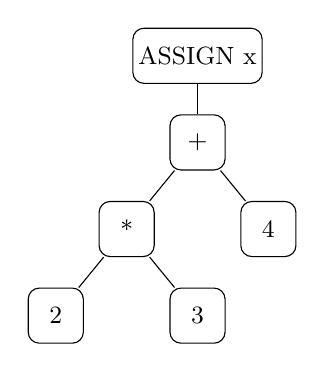
\begin{tikzpicture}[level distance=11mm, sibling distance=18mm, font=\small,
  every node/.style={draw,rounded corners,inner sep=2pt,minimum size=7mm}]
\node {\code{ASSIGN x}}
  child {node {\code{+}}
    child {node {\code{*}}
      child {node {2}}
      child {node {3}}
    }
    child {node {4}}
  };
\end{tikzpicture}
\caption{AST de l'instruction \code{x = 2 * 3 + 4}.}
\label{fig:ast-assign}
\end{figure}

Les listes de paramètres et d'arguments sont accumulées dans une petite structure
jetable \code{NodeList}, dont le tableau interne est ensuite transféré dans le
n\oe ud final (\code{NODE\_FUNC\_DECL} ou \code{NODE\_FUNC\_CALL}), puis seule la
coquille est libérée, une subtilité mémoire que Valgrind a confirmée sans fuite.

\subsection{L'évaluateur}

L'évaluateur réalise le parcours décrit au listing~\ref{lst:eval-pseudo}. Les
ruptures de flot non locales (retour de fonction, \code{arrêter}, \code{continuer})
sont gérées par des drapeaux globaux que les blocs et les boucles surveillent. Le
traitement d'un appel de fonction illustre la gestion de la pile d'environnements :

\begin{lstlisting}[style=c,caption={Appel de fonction : ordre d'évaluation et pile (extrait de \code{eval.c}).}]
/* 1) Evaluer les arguments dans l'environnement de l'APPELANT. */
for (i = 0; i < node->nargs; i++) argvals[i] = eval(node->args[i]);
/* 2) Empiler un nouveau frame et y lier les parametres. */
env_push();
for (i = 0; i < decl->nargs; i++) env_set(decl->args[i]->name, argvals[i]);
/* 3) Evaluer le corps, recuperer la valeur de retour. */
return_flag = 0; eval(decl->body);
result = return_flag ? return_value : make_int(0);
/* 4) Depiler le frame. */
env_pop();
\end{lstlisting}

L'ordre est crucial : les arguments sont évalués \emph{avant} l'empilement du
nouveau frame, faute de quoi une expression comme \code{fib(n-1)} chercherait
\code{n} dans le frame vide de la fonction appelée.

Le c\oe ur du calcul arithmétique se trouve dans \code{eval\_binop}, qui applique
la règle de cohabitation entiers/flottants. En voici un extrait commenté :

\begin{lstlisting}[style=c,caption={Cohabitation entiers/flottants et garde-fou (extrait de \code{eval.c}).}]
Value a = eval(node->left);
Value b = eval(node->right);
int both_int = (a.type == VAL_INT && b.type == VAL_INT);
switch (node->op) {
case OP_ADD:                       /* si deux entiers -> entier */
    return both_int ? make_int(a.ival + b.ival)
                    : make_float(as_double(a) + as_double(b)); /* sinon flottant */
case OP_DIV:
    if (both_int) {
        if (b.ival == 0) {         /* division entiere par zero : */
            fprintf(stderr, "Erreur ligne %d : division par zero\n", node->line);
            return make_int(0);    /* message emis, le programme continue */
        }
        return make_int(a.ival / b.ival);  /* division ENTIERE preservee */
    }
    /* ... cas flottant ... */
}
\end{lstlisting}

\paragraph{Exemple : trace d'exécution de \code{fib(3)}.} Pour rendre concret le
mécanisme d'appel récursif et de pile d'environnements, déroulons l'évaluation de
\code{fib(3)} avec la définition usuelle. Le tableau~\ref{tab:trace-fib} montre
l'enchaînement des appels, l'état du sommet de pile et la valeur retournée.

\begin{table}[ht]
\centering
\caption{Trace simplifiée de l'évaluation de \code{fib(3)}.}
\label{tab:trace-fib}
\small
\begin{tabular}{@{}llll@{}}
\toprule
\textbf{Appel} & \textbf{\code{n}} & \textbf{Action} & \textbf{Retour} \\
\midrule
\code{fib(3)} & 3 & $n \geq 2$ : calcule \code{fib(2)+fib(1)} & 2 \\
\quad\code{fib(2)} & 2 & $n \geq 2$ : calcule \code{fib(1)+fib(0)} & 1 \\
\quad\quad\code{fib(1)} & 1 & $n < 2$ : \code{retourner(1)} & 1 \\
\quad\quad\code{fib(0)} & 0 & $n < 2$ : \code{retourner(0)} & 0 \\
\quad\code{fib(1)} & 1 & $n < 2$ : \code{retourner(1)} & 1 \\
\bottomrule
\end{tabular}
\end{table}

Chaque ligne indentée correspond à un \code{env\_push} (nouveau frame avec son
propre \code{n}) suivi, au retour, d'un \code{env\_pop}. Le drapeau de retour
(\code{return\_flag}) est levé par \code{retourner} et « consommé » par la boucle
d'appel, qui récupère alors \code{return\_value}. Le résultat final, \code{fib(3) =
2}, est conforme à l'exécution réelle (cf. chapitre~\ref{chap:validation}).

\section{Aspects techniques notables}

\subsection{Le type \code{Value} : faire cohabiter entiers et flottants}

L'extension des flottants a transformé le type des valeurs manipulées. Plutôt que
de tout passer en \code{double} (ce qui aurait cassé la division entière et le
modulo), une \emph{union étiquetée} distingue les deux natures :

\begin{lstlisting}[style=c,caption={Le type \code{Value} (extrait de \code{ast.h}).}]
typedef enum { VAL_INT, VAL_FLOAT } ValType;
typedef struct Value { ValType type; long ival; double fval; } Value;
\end{lstlisting}

La règle sémantique est simple : une opération entre deux entiers reste entière ;
dès qu'un flottant intervient, le calcul bascule en \code{double}. Ainsi
\code{10 / 4} vaut \code{2} (sémantique d'origine préservée) tandis que
\code{10.0 / 4} vaut \code{2.5}.

\subsection{La portée lexicale}

Chaque environnement est une table de hachage de 211 alvéoles (un nombre premier,
pour mieux répartir les collisions), indexée par la fonction \code{djb2} de Dan
Bernstein :

\begin{lstlisting}[style=c,caption={Fonction de hachage djb2 (extrait de \code{symtab.c}).}]
static unsigned int hash(const char *s) {
    unsigned int h = 5381;
    int c;
    while ((c = (unsigned char)*s++) != 0)
        h = ((h << 5) + h) + c;   /* h * 33 + c */
    return h % HASH_SIZE;
}
\end{lstlisting}

La résolution d'une variable se fait dans le frame courant puis, en repli, dans
l'environnement global, \emph{sans} traverser les frames intermédiaires de la pile
d'appel. C'est ce qui garantit une portée \textbf{lexicale} : une fonction ne voit
jamais les variables locales de la fonction qui l'a appelée. Ce point a fait
l'objet d'une correction après une première version (involontairement) à portée
dynamique, détaillée au chapitre~\ref{chap:discussion}.

\paragraph{Exemple : la table des symboles pendant \code{pgcd(48, 18)}.} Lors de
l'appel à la fonction \code{pgcd}, un frame est empilé contenant les paramètres
\code{a} et \code{b}, auxquels s'ajoute la variable locale \code{temp} créée par
la première affectation. Le tableau~\ref{tab:pgcd-frame} montre l'évolution du
contenu de ce frame au fil des itérations de la boucle \code{tant que}.

\begin{table}[ht]
\centering
\caption{Évolution du frame de \code{pgcd} (algorithme d'Euclide sur 48 et 18).}
\label{tab:pgcd-frame}
\begin{tabular}{@{}cccc@{}}
\toprule
\textbf{Itération} & \code{a} & \code{b} & \code{temp} \\
\midrule
entrée   & 48 & 18 & (non créé) \\
1        & 18 & 12 & 18 \\
2        & 12 & 6  & 12 \\
3        & 6  & 0  & 6 \\
\midrule
\multicolumn{4}{c}{$b = 0$ : sortie de boucle, \code{retourner(a)} $\Rightarrow$ \textbf{6}} \\
\bottomrule
\end{tabular}
\end{table}

\subsection{Localisation des erreurs à la ligne}

Tous les messages d'erreur indiquent la ligne fautive, au format
\code{Erreur ligne N : ...}. Le choix de conception décisif est de \emph{figer le
numéro de ligne dans chaque n\oe ud au moment du parsing}
(\code{node->line = yylineno} dans le constructeur), et non à l'évaluation. En
effet, au moment où l'évaluation commence, l'analyse lexicale est terminée :
\code{yylineno} vaut alors la \emph{dernière} ligne du fichier. L'utiliser dans
l'évaluateur ferait pointer toutes les erreurs sur la fin du fichier. En gravant
la ligne dans le n\oe ud à sa création, chaque diagnostic d'exécution désigne le
bon emplacement, comme le confirme le test du « mauvais nombre d'arguments », qui
signale correctement la ligne~5, celle de l'appel fautif, et non la fin du
fichier.

\subsection{Les optimisations et le garde-fou de la division par zéro}

Le pliage de constantes calcule à la compilation les sous-expressions
entièrement constantes. Un piège guette : \code{10 / 0} est, lui aussi, composé de
deux littéraux. Le plier provoquerait soit un \code{SIGFPE} pendant la
compilation, soit un court-circuitage du message d'erreur attendu à l'exécution.
Une fonction \code{can\_fold} interdit donc de plier toute division ou modulo qui
échouerait ; ces cas restent dans l'arbre et c'est l'évaluateur qui émet le
diagnostic.

\begin{lstlisting}[style=c,caption={Garde-fou du pliage (extrait de \code{optim.c}).}]
static int can_fold(int op, Value a, Value b) {
    int both_int = (a.type == VAL_INT && b.type == VAL_INT);
    if (op == OP_DIV) return both_int ? (b.ival != 0) : (as_double(b) != 0.0);
    if (op == OP_MOD) return both_int && (b.ival != 0); /* modulo : entiers, != 0 */
    return 1;   /* toutes les autres operations sont pliables */
}
\end{lstlisting}

\paragraph{Exemple : avant/après pliage.} Sur l'expression \code{2 + 3 * 4},
l'optimiseur reconnaît que \code{3 * 4} a deux fils littéraux et le remplace par
\code{12}, puis que \code{2 + 12} est à son tour pliable, et le remplace par
\code{14}. L'arbre de gauche (figure~\ref{fig:fold}) est ainsi réduit à une
unique feuille. À l'exécution, \code{afficher(2 + 3 * 4)} n'effectue donc
\emph{aucun} calcul : la valeur 14 est déjà dans l'arbre.

\begin{figure}[ht]
\centering
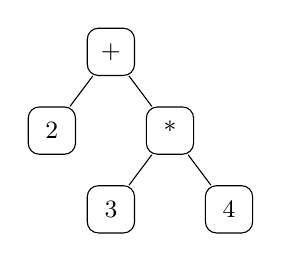
\begin{tikzpicture}[level distance=10mm, sibling distance=15mm, font=\small,
  every node/.style={draw,rounded corners,inner sep=2pt,minimum size=6mm}]
\node {\code{+}}
  child {node {2}}
  child {node {\code{*}}
    child {node {3}}
    child {node {4}}
  };
\end{tikzpicture}
\hspace{1.5cm}
\raisebox{1.2cm}{$\xrightarrow{\text{ pliage }}$}
\hspace{1.5cm}
\raisebox{1.0cm}{%
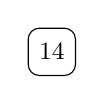
\begin{tikzpicture}[font=\small, every node/.style={draw,rounded corners,inner sep=2pt,minimum size=6mm}]
\node {14};
\end{tikzpicture}}
\caption{Pliage de constantes : l'arbre de \code{2 + 3 * 4} est réduit à la
feuille \code{14}.}
\label{fig:fold}
\end{figure}

De même, l'élimination du code mort transforme \code{si (0) \{ A \} sinon \{ B \}}
en le seul bloc \code{B}, et \code{si (1) \{ A \}} en le seul bloc \code{A}, la
condition constante étant évaluée une fois pour toutes à la compilation.

\subsection{Gestion de la mémoire}

L'AST est entièrement alloué dynamiquement, puis libéré récursivement par
\code{free\_node}. Le transfert du tableau d'arguments depuis la \code{NodeList}
vers le n\oe ud (sans le dupliquer ni le libérer deux fois) a demandé une
attention particulière. La vérification Valgrind confirme l'absence de fuite (voir
chapitre~\ref{chap:validation}), après ajout d'un appel à \code{yylex\_destroy()}
pour libérer le tampon interne de Flex.

\subsection{Sûreté et robustesse}

Bien qu'\ilang{} ne soit pas exposé à un contexte adverse, plusieurs propriétés de
\emph{sûreté} ont été soignées. La mémoire est intégralement maîtrisée :
allocations vérifiées (tout \code{malloc}/\code{realloc} dont l'échec est fatal
est testé), libération récursive de l'AST, et absence de fuite confirmée par
Valgrind. Aucune entrée utilisateur n'est copiée dans un tampon de taille fixe :
les identifiants sont dupliqués par \code{strdup} (allocation dimensionnée), ce
qui exclut tout débordement de tampon à l'analyse. Les conditions d'erreur
(variable ou fonction indéfinie, mauvais nombre d'arguments, division par zéro,
rupture de flot hors boucle, caractère ou syntaxe invalides) sont toutes
interceptées et signalées plutôt que de produire un comportement indéfini
silencieux. La seule limite de sûreté identifiée est le débordement de la pile de
l'hôte en cas de récursion très profonde (cf. chapitre~\ref{chap:validation}),
inhérent à l'évaluation récursive.

\subsection{Le back-end assembleur (extension hors-périmètre)}

Le module \code{codegen.c} parcourt le même AST mais émet du code assembleur i386
(syntaxe AT\&T) au lieu d'évaluer. Il applique la convention d'appel cdecl :
arguments empilés de droite à gauche, résultat dans \code{\%eax}, cadre de pile
géré par \code{\%ebp}/\code{\%esp}. Les variables du programme principal deviennent
des globales en \code{.bss}, les paramètres et locales des fonctions sont rangés
en déplacement par rapport à \code{\%ebp}. Les expressions sont compilées en
machine à pile. Ce module, entièrement optionnel, n'altère en rien
l'interpréteur ; il est décrit en détail au chapitre~\ref{chap:discussion} et son
code figure en annexe~\ref{annexe:code}.

La traduction d'une opération binaire illustre la stratégie de machine à pile :

\begin{lstlisting}[style=c,caption={Génération d'un binop en machine à pile (extrait de \code{codegen.c}).}]
gen_expr(out, n->left);                 /* operande gauche -> %eax */
fprintf(out, "\tpushl %%eax\n");        /* sauvegarde sur la pile */
gen_expr(out, n->right);                /* operande droit  -> %eax */
fprintf(out, "\tmovl %%eax, %%ecx\n");  /* droit  -> %ecx */
fprintf(out, "\tpopl %%eax\n");         /* gauche -> %eax (restaure) */
switch (n->op) {
case OP_ADD: fprintf(out, "\taddl %%ecx, %%eax\n"); break;  /* eax = eax + ecx */
case OP_MUL: fprintf(out, "\timull %%ecx, %%eax\n"); break;
/* division : cltd etend le signe, idivl place le quotient dans %eax */
case OP_DIV: fprintf(out, "\tcltd\n\tidivl %%ecx\n"); break;
}
\end{lstlisting}

\paragraph{Exemple : assembleur produit pour une fonction.} Pour la fonction
\code{fonction carre(x) \{ retourner(x * x) \}}, le générateur produit le code du
listing~\ref{lst:asm-carre}, ici annoté. On y reconnaît le prologue cdecl, l'accès
au paramètre par déplacement positif depuis \code{\%ebp}, la machine à pile pour
le produit, et l'épilogue.

\begin{lstlisting}[style=asm,caption={Assembleur généré pour \code{carre} (annoté).},label={lst:asm-carre}]
il_carre:
    pushl %ebp            # prologue : sauvegarde l'ancien base pointer
    movl %esp, %ebp       # etablit le nouveau cadre de pile
    movl 8(%ebp), %eax    # charge le parametre x (1er arg en +8)
    pushl %eax            # empile x (operande gauche)
    movl 8(%ebp), %eax    # recharge x (operande droit)
    movl %eax, %ecx       # x -> %ecx
    popl %eax             # x -> %eax
    imull %ecx, %eax      # %eax = x * x
    leave                 # epilogue : restaure %esp et %ebp (retourner)
    ret                   # retour, resultat dans %eax
\end{lstlisting}

Côté appelant, \code{afficher(carre(7))} empile la constante 7, appelle
\code{il\_carre}, nettoie la pile (\code{addl \$4, \%esp}), puis transmet le
résultat (\code{\%eax}) à \code{printf} via le format \code{"\%d\textbackslash n"}.
Cette correspondance directe entre les concepts de l'évaluateur (pile d'appels,
liaison des paramètres) et leur réalisation matérielle (cadre \code{\%ebp},
déplacements) est précisément ce que le chapitre~2 du cours cherche à faire
comprendre.

\paragraph{Traduction des boucles.} Les structures de contrôle deviennent des
\emph{labels} et des \emph{sauts}. Une boucle \code{tant que (c) \{ corps \}} est
encadrée par deux labels : un label de tête (avant le test) et un label de fin.
La condition échouée saute vers la fin ; le corps se termine par un saut
inconditionnel vers la tête. Les instructions \code{arrêter} et \code{continuer}
se traduisent alors trivialement par un \code{jmp} vers, respectivement, le label
de fin et le label de tête (ou d'incrément pour une boucle \code{pour}). Le
générateur maintient à cet effet une pile de labels de boucles, exactement comme
l'évaluateur maintient un signal de rupture. Schématiquement :

\begin{lstlisting}[style=asm,caption={Schéma de traduction d'une boucle \code{tant que}.}]
.Ltete:                  # etiquette de tete
    < code de la condition c, resultat dans %eax >
    cmpl $0, %eax
    jz .Lfin             # si c est faux -> sortir
    < code du corps >    # 'arreter' = jmp .Lfin ; 'continuer' = jmp .Ltete
    jmp .Ltete           # boucler
.Lfin:                   # etiquette de fin
\end{lstlisting}

\subsection{Compilation automatisée}

Le \code{Makefile} sépare deux jeux d'options : le code du projet est compilé avec
\code{-Wall -Wextra} (zéro avertissement exigé), tandis que le code engendré par
Flex et Bison est compilé sans \code{-Wextra}, ces fichiers machine-générés
pouvant contenir des constructions qui déclencheraient des avertissements non
imputables au projet. Les dépendances entre fichiers générés (\code{lex.yy.c}
dépend de \code{ilang.tab.h}) sont explicitées pour que \code{make} ordonne
correctement la compilation.

\begin{lstlisting}[style=gram,caption={Séparation des jeux d'options (extrait du \code{Makefile}).}]
CFLAGS   = -Wall -Wextra -std=gnu11 -g    # notre code : tous les avertissements
GENFLAGS = -std=gnu11 -g                  # code genere : sans -Wextra

# Bison : grammaire -> parseur + en-tete des tokens
ilang.tab.c ilang.tab.h: ilang.y
	$(YACC) -d -o ilang.tab.c ilang.y
# Flex : depend de l'en-tete des tokens engendre par Bison
lex.yy.c: ilang.l ilang.tab.h
	$(LEX) -o lex.yy.c ilang.l
\end{lstlisting}

Le point d'entrée \code{main.c} se charge enfin d'analyser les arguments (chemin
du fichier, options \code{-s} et \code{--no-opt}), d'enchaîner
\code{yyparse()} $\to$ \code{optimize()} $\to$ \code{eval\_program()} (ou
\code{generate\_asm()}), puis de libérer l'AST et la table des symboles avant de
rendre la main.
